\documentclass[sigconf,review]{acmart}
\usepackage{tikz}
\usepackage{tikzsymbols}

\setcopyright{none}

\begin{document}
\title{Bluesky and the AT Protocol: Usable Decentralized Social Media}
\author{Martin Kleppmann}
\email{martin@kleppmann.com}
\orcid{0000-0001-7252-6958}
\affiliation{%
  \institution{TU Munich}
  \city{Munich}
  \country{Germany}
}

\author{TODO: review author list}
\author{Paul Frazee, Jake Gold, Jay Graber}
\author{Daniel Holmgren, Devin Ivy, Jeromy Johnson}
\author{Bryan Newbold, Jaz Volpert}
\affiliation{%
  \institution{Bluesky PBC}
  \country{United States}
}

\begin{abstract}
TODO
% an architecture inspired by the web itself, but modernized to include streams of real-time updates and cryptographic authentication.
\end{abstract}

\begin{CCSXML}
<ccs2012>
   <concept>
       <concept_id>10002951.10003260.10003282.10003292</concept_id>
       <concept_desc>Information systems~Social networks</concept_desc>
       <concept_significance>500</concept_significance>
   </concept>
   <concept>
       <concept_id>10003033.10003106.10003114.10003118</concept_id>
       <concept_desc>Networks~Social media networks</concept_desc>
       <concept_significance>500</concept_significance>
   </concept>
   <concept>
       <concept_id>10003456.10003457.10003490.10003507.10003508</concept_id>
       <concept_desc>Social and professional topics~Centralization / decentralization</concept_desc>
       <concept_significance>300</concept_significance>
   </concept>
 </ccs2012>
\end{CCSXML}

\ccsdesc[500]{Information systems~Social networks}
\ccsdesc[500]{Networks~Social media networks}
\ccsdesc[300]{Social and professional topics~Centralization / decentralization}

\keywords{social media, decentralization, federation, web architecture}
\maketitle

\section{Introduction}

Over the last two decades, social media services have evolved from a fun curiosity into a cornerstone of civic life~\cite{Barabas:2017}.
This development has been accompanied by increasing unease that mainstream ``digital town squares'', such as Twitter/X or Facebook, are under the control of a single corporation, and may change their policies on the whim of their leaders~\cite{Yeung:2023}.
Their operations are opaque (e.g.\ regarding which content is recommended to users), and their users lack agency over their user experience.
As a result, there has been increasing interest in decentralized social networks, of which the \emph{fediverse} around the ActivityPub protocol~\cite{ActivityPub} and the Mastodon software~\cite{Mastodon} is perhaps the best known (we review a selection of decentralized social networks in Section~\ref{sec:related-work}).

However, decentralization also introduces new challenges.
For example, in the case of Mastodon, a user needs to choose a server when creating an account.
This choice is significant because the server name becomes part of the username; migrating to another server implies changing username, and preserving one's followers during such a migration requires the cooperation of the old server.
If a server is shut down without warning, accounts on that server cannot be recovered~-- a particular risk with volunteer-run servers.
In principle, a user can host their own server, but only a small fraction of social media users have both the technical skills and the inclination to do so.

The distinction between servers in Mastodon introduces complexity for users that does not exist in centralized services.
For example, a user viewing a thread of replies in the web interface of one server may see a different set of replies compared to viewing the same thread on another server, because a server only shows those replies that it knows about~\cite{Adida:2022}.
As another example, when viewing the web profile of an account on another server, clicking the ``follow'' button does not simply follow that account; instead, the user needs to enter the hostname of their own server and be redirected to a URL on their home server before they can follow the account.
In our opinion, it is undesirable to burden users with such complexity arising from the federated architecture.

In this paper we introduce the \emph{AT Protocol} (atproto), a decentralized foundation for social networking, and \emph{Bluesky}, a Twitter-style social app built upon it.
A core design goal of atproto and Bluesky is to enable a user experience of the same or better quality as centralized services, while being open and decentralized on a technical level.
We introduce the user-facing features of Bluesky in Section~\ref{sec:product}, and in Section~\ref{sec:architecture} we explain the underlying systems architecture.
The AT Protocol is designed such that for every part of the system there are multiple competing operators providing interoperable services, making it easy to switch from one provider to another.

Decentralization alone is not able to solve some of the thorniest problems of social media, such as misinformation, harassment, and hate speech.
However, by opening up the internals of a service to contributors who are not employees of a particular company, decentralization can enable a marketplace of approaches to these problems.
For example, Bluesky allows anybody to create custom feeds that can apply arbitrary filtering and content selection methods, and custom client software can access all features of the ``official'' app, including moderation tools.
Our hope is that this architectural openness will enable communities to develop their own approaches to managing problematic content, without depending on a centralized service operator to implement these features for them.

For example, researchers wanting to identify disinformation campaigns can easily get access to all content being posted, the social graph, and user profiles on Bluesky.
If they are able construct an algorithm to label suspected disinformation, they can publish their labels in real time for use by other parts of the system, such as custom feed generators or client apps.
One goal of this paper is therefore to bring Bluesky and the AT Protocol to the attention of researchers working on such algorithms, and to invite them to use the rapidly growing dataset of Bluesky content as a basis for their work.

\section{The Bluesky Social App}\label{sec:product}

Bluesky presents itself to users as a straightforward microblogging application in the style of Twitter/X (see Figure~\ref{fig:home-feed}).
The ``official'' client app is available on iOS, Android, and the web; several independently developed client apps are also available, such as Graysky and deck.blue. % TODO: links to those apps
Users can make public posts containing up to 300 characters of text, and up to four images, and they can interact with posts by replying, reposting, or liking.
A user can also follow other users, and the default feed shows posts by accounts that the user is following in reverse chronological order.
There are also alternative feeds that show content on various topics, without the user needing to follow the poster (see Section~\ref{sec:feeds}), which helps users discover each other.

\begin{figure}
    \centering
    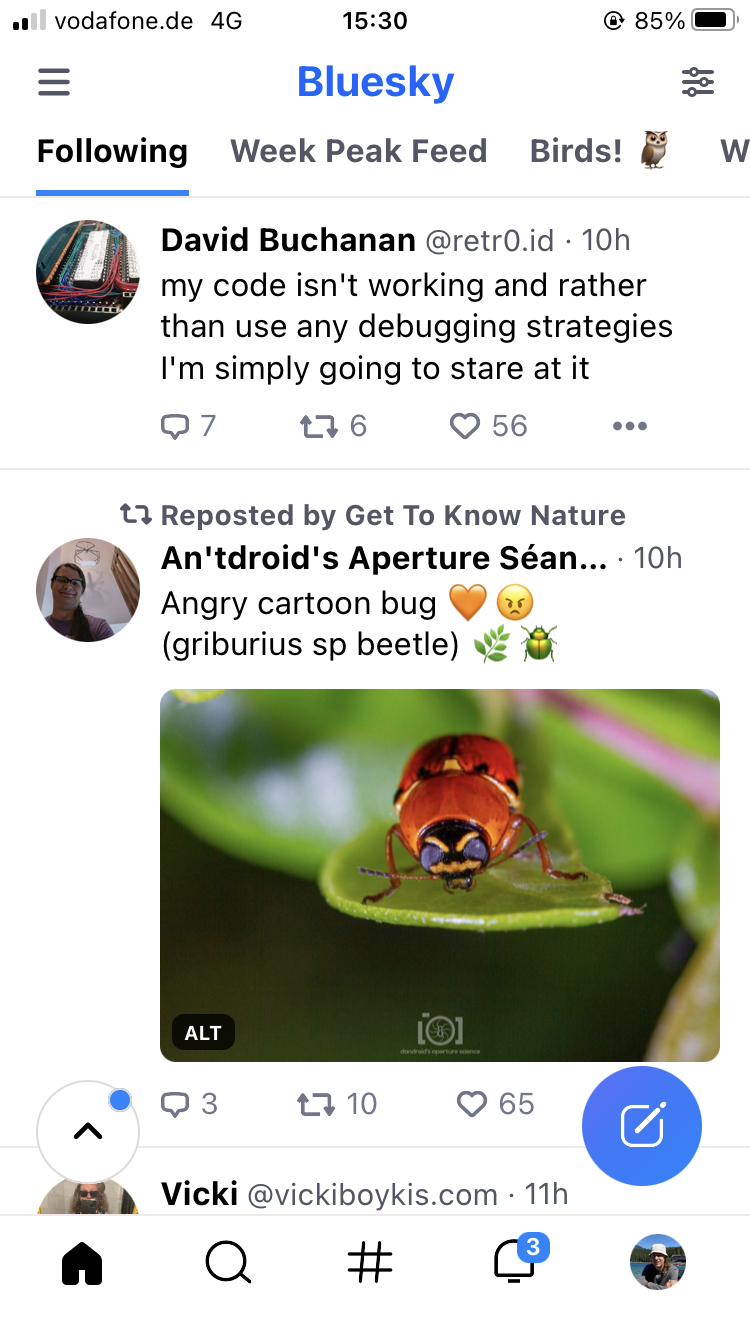
\includegraphics[width=0.7\linewidth]{home-feed.png}
    \Description{A Twitter-like feed of short posts. At the top is a feed selector, in which the default ``Following'' feed is active.}
    \caption{Screenshot of the Bluesky home screen.}
    \label{fig:home-feed}
\end{figure}

\begin{figure}
    \centering
    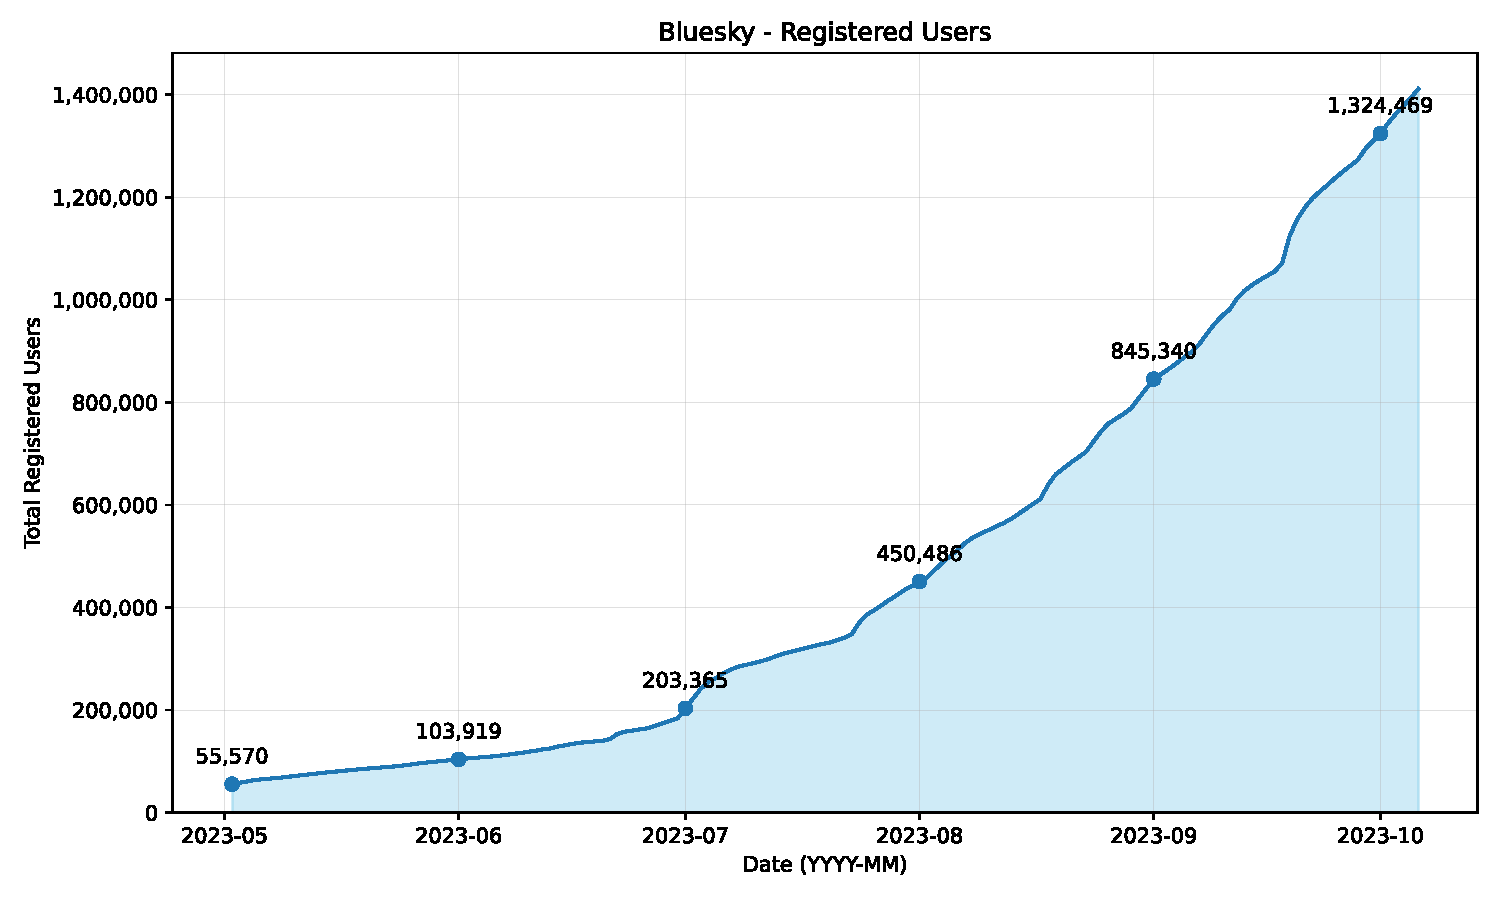
\includegraphics[width=\linewidth]{user-growth.pdf}
    \Description{An exponential growth curve, approximately doubling every month, starting at 55k in May 2023 and exceeding 1.3M in October 2023.}
    \caption{Number of registered Bluesky users from May to October 2023.}
    \label{fig:user-growth}
\end{figure}

Bluesky launched an invite-only beta release in February 2023, and has grown to over 1.5~million registered users in October 2023, as shown in Figure~\ref{fig:user-growth}.
At the time of writing, an invitation code is required to create an account, and codes are available through a waitlist or from an existing user.
Such control over user signups may seem contradictory for a supposedly open and decentralized network, but it has been necessary to limit the load on our infrastructure and to keep abuse at a manageable level.
We intend to remove the need for invite codes in early 2024.

Bluesky, PBC (a public-benefit corporation) develops the official client app and operates the core services; the client and several server-side components are open source under the MIT license~\cite{BlueskyGithub}.
The protocols they use are defined by open specifications~\cite{AtProtoSpecs}.
Several parts of the system, such as feed generators (Section~\ref{sec:feeds}) and various alternative clients~\cite{AtProtoClients} are developed and operated by independent third parties.

\subsection{Moderation Features}\label{sec:moderation}

Bluesky has several moderation mechanisms for managing unwanted content:
\begin{description}
    \item[Content filtering:] Automated systems label potentially problematic content (such as images of a sexual or violent nature, posts promoting hate groups, or spam), and the app's preferences allow users to choose whether to show or hide content in each of these categories in their feeds.
    \item[Mute:] A user can mute specific accounts or threads, which hides the muted content from their own feeds and notifications. The content continues to be visible to other users, and the target does not know that they were muted. A user can also publish a mutelist of accounts, and other users can subscribe to that list, which has the same effect as if they individually muted all of the accounts on the list.
    \item[Block:] One user can block another, which prevents all future interactions (such as mentions, replies, or reposts) between those accounts in addition to muting.
    \item[Takedown:] Users can report content that violates the terms of service to server operators, and the operators can take down violating posts or accounts.
    \item[Custom feeds:] While the aforementioned mechanisms provide negative moderation (helping users avoid content they do not want to see), feed generators (see Section~\ref{sec:feeds}) can actively select high-quality content.
\end{description}

Additional moderation mechanisms are under discussion~\cite{Moderation}.

\subsection{User Handles}\label{sec:handles}

Like on Twitter, a Bluesky user has two names: the \emph{display name} can be almost any string, and the \emph{handle} needs to uniquely identify a user.
A handle, prefixed with an @ sign, is used to mention another user in a post.
Examples can be seen in Figure~\ref{fig:home-feed} (the display name is in bold, and the handle is in a smaller font and lighter color).

The need for handles to be unique creates challenges in decentralized systems, since it requires an authority that determines which handle is assigned to which user.
Mastodon's approach is to include the server name in the handle, which makes it difficult to move to another server.
An alternative would be to use a blockchain-based naming system, such as the Ethereum Name System (ENS)~\cite{ENS}; this has the disadvantage of requiring the user to buy cryptocurrency in order to create an account, which we wanted to avoid.

Instead, Bluesky and atproto use DNS domain names as handles.
If a user already owns a domain name, they can claim it as their Bluesky handle by adding a DNS record or by hosting a file under a \texttt{.well-known} HTTPS URL on that domain~\cite{DomainHandle}.
Users can also buy a new domain name within Bluesky, via a partnership with a domain registrar~\cite{PurchaseDomain}.
Alternatively, users can sign up for a subdomain of \texttt{.bsky.social} for free.

Using DNS domain names as handles has several advantages:
\begin{itemize}
    \item We leverage the existing infrastructure of ICANN, registrars, and name servers, including for example the dispute resolution procedures for trademarks.
    \item Domain names are a well-known concept even among non-technical users, and they are short and simple.
    \item A user can move to a different server without changing their handle.
    \item Users do not need to host their own server to use their own domain name; a DNS record requires only a one-time setup and no ongoing maintenance.
    \item For organizations and people that already have a well-known domain name, using that name makes it easy for users to check that their Bluesky account is genuine. For example, the New York Times' handle is \texttt{@nytimes.com}.
    \item An organization can easily allow their staff to demonstrate their affiliation by granting them handles that are subdomains of the organization's main domain name (comparable to institutional email addresses). For example, a journalist's handle may indicate that they are at a particular news organization.
    \item Providers wanting to offer free subdomains can do so at very little cost.
\end{itemize}

\subsection{Custom Feeds and Algorithmic Choice}\label{sec:feeds}

Several decentralized social networks choose to offer only a reverse-chronological feed of posts from accounts the user is following~-- a backlash against the opaque content recommendation algorithms employed by mainstream centralized social networks.
For example, Mastodon advertises itself as having ``no algorithms or ads to waste your time''~\cite{Mastodon}.

Our belief is that the problem lies not with algorithms \emph{per se}, but rather with centrally controlled, opaque algorithms that remove user agency and prioritize user engagement over all else, e.g.\ by promoting controversial posts.
Good recommendation algorithms can help users discover content that is relevant to them and find new accounts to follow~-- especially important for new users who are not yet following many accounts.
They are also helpful for surfacing content on a particular topic, whereas following a user means seeing all of their posts, which might be on a mixture of topics, not all necessarily interesting to all followers.

Bluesky, PBC offers a selection of feed generation algorithms of its own, and also allows anybody to create their own feed generator~\cite{CustomFeeds}.
The goal is to offer an open and diverse ``marketplace of algorithms'' in which communities can adapt the system to suit their needs, and users have more agency over how they spend their time and attention~\cite{AlgorithmicChoice}.
TODO: how many custom feeds have been created to date? link to section about how feed generators work.

In Figure~\ref{fig:home-feed}, a selection of bookmarked feeds is given at the top of the screen; in this example, the selected ``Following'' feed is the default reverse-chronological timeline, while ``Week Peak Feed'' (network-wide posts with many likes from the last week) and ``Birds!'' (photos and posts from birdwatchers) are third-party feeds.
A feed generator can use arbitrary criteria to select its content.
For example, the birdwatching feed uses manual review of accounts in combination with a \#birds hashtag or a feather emoji character in posts to identify posts to include.
Alternative approaches, such as machine learning algorithms, are equally possible.

\begin{figure*}
    \centering
    
\begin{tikzpicture}
        \node (user) at (0,0) {\Strichmaxerl[5]};
        \node (pds1) at (2,0) {PDS 1};
    \end{tikzpicture}
    \caption{The main services involved in providing Bluesky, and their relationships.}
    \label{fig:indexing}
\end{figure*}

\section{The AT Protocol Architecture}\label{sec:architecture}

Bluesky is the social app with the features explained in Section~\ref{sec:product}, while the AT Protocol is the underlying decentralized foundation.
We maintain this separation because the AT Protocol is designed to support multiple social apps, not just Bluesky.
For example, besides a Twitter-style microblogging app, atproto could also be used to implement Reddit-style forums, long-form blogs with comments, or domain-specific social applications such as link sharing or book reviews.
The same user identity, social graph, and user data storage servers can be shared between all of these apps.

The main constraint is that atproto is designed for content that users intend to make publicly available.
In particular, Bluesky user profiles, posts, follows, and likes are all public.
Blocking actions are also currently public; however, we are investigating mechanisms for making these private~\cite{PrivateBlocks}.
At present, Bluesky does not support direct messages, which would need to be private and encrypted.
Only a small amount of Bluesky user state is currently private: any muted accounts and threads, notifications, and their read/unread status.

\subsection{User Data Repositories}\label{sec:repos}

All data that a user wishes to publish is added to their \emph{repository}, which stores a collection of \emph{records}.
Whenever a user performs some action~-- making a post, liking another user's post, following another user, etc.~-- that action becomes a record in their repository.
Each user account has one repository, and it contains all of the actions they have ever performed, minus any records they have explicitly deleted.
A \emph{Personal Data Server (PDS)} hosts the user's repository and makes it publicly available as a web service; we discuss PDSes in more detail in Section~\ref{sec:pds}.

A user only updates their own repository; for example, if user $A$ follows user $B$, this results only in a follow record in user $A$'s repository, and no change to $B$'s repository.
To find all followers of user $B$ requires indexing the content of all repositories.
This design decision is similar to the way hyperlinks work on the web: it is easy to find all the outbound links from a web page at a given URL, but to find all the inbound links to a page requires an index of the entire web, which is maintained by web search engines.

The \emph{AT} in atproto stands for \emph{Authenticated Transfer}, which reflects the fact that repositories are cryptographically authenticated.
The records in a repository are organized into a \emph{Merkle Search Tree} (MST), a type of Merkle tree that remains balanced, even as records are inserted or deleted in arbitrary order~\cite{Auvolat:2019}.
After every change to a repository, the root hash of the MST is signed; the public verification key for this signature is part of the user identity described in Section~\ref{sec:identity}.
This enables an efficient cryptographic proof that a given record appears within a given user's repository.

\subsection{Personal Data Servers (PDS)}\label{sec:pds}

A PDS allows anybody to query the content of the repositories that it hosts via a HTTP API.
Moreover, a PDS provides a real-time stream of updates for the repositories it hosts.
Indexers (see Section~\ref{sec:indexing}) subscribe to this stream in order to find out about new records (posts, likes, follows, etc.) with low latency.

Since a PDS only deals with the data generated by the users it hosts, a PDS for a small number of users requires only small computing resources, even if those users have a large number of followers.
Users who wish to self-host their own PDS can therefore do so on a cheap virtual machine in the cloud, or even on a Raspberry Pi connected to their home internet router.
However, we expect that most users will sign up for an account on a shared PDS run by a professional hosting provider~-- either Bluesky, PBC, or another company.

Compared to choosing a Mastodon server, the user's choice of PDS hosting provider is fairly inconsequential.
The PDS URL is internal to the system, and is not normally visible to users.
It makes no difference whether two users are on the same PDS or different PDSes, since interaction between users goes via the indexing infrastructure in any case.
A user can migrate from one PDS to another by simply copying their repository to the new PDS, and pointing their account ID at the new PDS URL (see Section~\ref{sec:identity}).
Even if a PDS shuts down without warning, users can upload a backup of their repository to a new PDS, and thus recover their account without losing any of their posts or their social graph.

PDS operators will generally want to perform some basic moderation by deleting any illegal content hosted on their servers.
However, PDS-level moderation is much less important than server-level moderation in Mastodon, because in atproto, the primary moderation role is taken on by seperate actors in the system~-- the labelers and feed generators (see Section~\ref{sec:labeling}).
This allows different sets of people to offer server hosting and moderation services, respectively; we believe this separation is valuable since operating a server and moderating a community require largely disjoint skill sets.

At the time of writing, Bluesky's indexing infrastructure (see Section~\ref{sec:indexing}) only accepts repositories on PDS instances hosted by Bluesky, PBC itself; like invitation codes, this limitation exists to limit infrastructure load and abuse problems during the private beta.
In that sense, Bluesky is not yet fully decentralized.
However, support for third-party PDS operators is already implemented and enabled in Bluesky's \emph{sandbox} (testing) environment, and a PDS implementation suitable for self-hosting is already open source~\cite{BlueskyGithub}.
Support for third-party PDS operators will be enabled at the latest when invitation codes are removed in early 2024.

\subsection{Indexing Infrastructure}\label{sec:indexing}

On the web, websites are crawled and indexed by search engines, which then provide web-wide search and discovery features that the websites alone cannot provide.
The AT Protocol is inspired by this architecture: the repositories hosted by PDSes are analogous to websites, and the indexing infrastructure is analogous to a search engine.
User repositories are primary data (the ``source of truth''), and the indexes are derived from the content of the repositories.

At the time of writing, most of Bluesky's indexing infrastructure is operated by Bluesky, PBC, but the company does not have any privileged access: since repositories are public, anybody can crawl and index them using the same protocols as our systems use.
Client apps can switch to reading from a different index, or use a combination of multiple indexes.
However, while operating a small PDS is designed to be cheap, operating an indexer that ingests the entire network requires greater computing resources.
We therefore expect that there will be fewer hobbyist indexers, but as Bluesky grows, there are likely to be multiple professionally-run indexers for various purposes.
For example, a company that performs sentiment analysis on social media activity about brands could easily create a whole-network index that provides insights to their clients.

The indexing infrastructure operated by Bluesky, PBC is illustrated in Figure~\ref{fig:indexing}.
It is composed of multiple services that have several integration points for external services.

\subsubsection{Big Graph Service (BGS)}\label{sec:bgs}

The first component is the \emph{Big Graph Service} (BGS), which crawls the user repositories on all known PDSes and consumes the streams of updates that they produce.
BGS checks the signatures and Merkle tree proofs on updates, and maintains its own replica of each repository.
From this information, BGS creates the \emph{firehose}: an aggregated stream of updates that notifies subscribers whenever records are added or deleted in any of the known repositories.

The firehose is publicly available.
Consuming the firehose is an easier way of building an index over the whole network, compared to directly subscribing to the source PDSes, since the BGS performs some initial data cleaning such as discarding malformed updates and filtering out high-volume spam.
The firehose can optionally include Merkle proofs and signatures along with records, allowing subscribers to check that they are authentic.

BGS does not interpret or index the records in repositories, but simply stores and forwards them.
Any developers wanting to create a new social app on top of atproto can define new record types, and these can be stored in existing repositories and aggregated in the firehose without requiring any changes to the BGS.

\subsubsection{The App View}\label{sec:appview}

The App View is a service that consumes the firehose, and processes the record types belonging to the Bluesky social app.
For example, the App View counts the number of likes on every post, and it collects the set of replies to a particular post.
The App View also maintains the set of followers for each user, and constructs the timeline containing the posts by the accounts that each user is following.
Finally, it offers a web service through which this information can be queried.

To display this information in the user's client app, the client queries the user's own PDS, which then fetches the neccessary data from the App View.
The PDS personalizes the information from the App View to include details that are specific to the querying user, e.g.\ hiding posts from accounts that the user has muted, and indicating whether the user has already liked a given post.

The App View is also responsible for enforcing moderation controls; for example, if one user has blocked another, the App View drops any attempts by the blocked users to interact with each other.
If users are unhappy with the moderation rules applied by the App View operated by Bluesky, PBC, it is always possible for third parties to operate alternative App Views that index the same firehose and present the data in a different way.

If the AT Protocol is used to implement another social application besides microblogging, that application will most likely require an App View service of its own, which can be hosted by anyone.
This service can then interpret and index the records in users' repositories in whatever way is required for that application.

\subsection{Labelers and Feed Generators}\label{sec:labeling}

\subsection{User Identity}\label{sec:identity}

% Labeling services https://github.com/bluesky-social/proposals/tree/main/0002-labeling-and-moderation-controls

% Federation architecture https://blueskyweb.xyz/blog/5-5-2023-federation-architecture

\subsection{TODO}

How are images stored? When migrating an account to a new PDS, presumably images need to be moved along with the repo. Do viewers of an image fetch it from the PDS of the user who posted it, or from the App View?

How does a PDS operator take down a ToS-violating post within a repo? Do they directly modify the repo and sign a new commit? How would this work if the signing key is not held custodially by the PDS, but rather by a client-side wallet?

Do blocklists exist yet?

Are keys held custodially by a PDS actually stored in a HSM? Is this why the same key is currently shared by all users on the same PDS? How will the key management change as a result of the PDS 2.0 architecture and the use of dedicated hardware in multiple locations?

Do we want to talk about some kind of robots.txt-like mechanism through which users can specify preferences regarding crawling and indexing?

\section{Related Work}\label{sec:related-work}

% https://activitypub.rocks/

% https://scuttlebutt.nz/
% https://github.com/lens-protocol/core
% https://nostr.com/
% "the Nostr protocol powers Minds and Snort, among other decentralized social media"

% https://www.farcaster.xyz/
% https://github.com/farcasterxyz/protocol/blob/main/docs/OVERVIEW.md
% https://www.varunsrinivasan.com/2022/01/11/sufficient-decentralization-for-social-networks

% for likes, the record is around 100 bytes, and the the MST tree stuff is anywhere from 1-4kb (depending on the repo and other randomness in the MST), usually averaging around 2.5Kb.
% https://github.com/bluesky-social/discuss/discussions/16#discussioncomment-7233086

\begin{acks}
TODO
\end{acks}

\bibliographystyle{ACM-Reference-Format}
\bibliography{references}
\end{document}
